\documentclass[
  11pt,
  letterpaper,
   addpoints,
   answers
  ]{exam}

\usepackage{../exercise-preamble}
\usepackage{float}
\usepackage{tikz}
\usepackage{cancel} % Para mostrar la sustitución sin(theta) -> theta
\usetikzlibrary{decorations.pathmorphing}

\begin{document}
\pagestyle{headandfoot}
\firstpagefooter{ }{Página \thepage\ de \numpages}{ }
\runningfooter{ }{Página \thepage\ de \numpages}{ }

\noindent
\begin{minipage}{0.47\textwidth}

\includegraphics[width=\textwidth]{../fcfm_die.png}
\end{minipage}
\begin{minipage}{0.53\textwidth}
\begin{center} 
\large\textbf{Introducción a la Física Moderna} (F1100) \\
\end{center}
\end{minipage}

\vspace{0.5cm}
\noindent
\vspace{.85cm}

\begin{questions}
%--------------------------
\question Un péndulo de longitud $L$ con una masa $M$ está unido lateralmente a un resorte de constante elástica $k$, como se muestra esquemáticamente. Cuando la masa cuelga verticalmente bajo el punto de suspensión, el resorte está sin deformación.
\begin{parts}
  \part Obtén una expresión aproximada para el período de oscilación del sistema para pequeñas amplitudes (linealiza las ecuaciones de movimiento).
  \part Supón $M=1{,}00\,\mathrm{kg}$ y que, en ausencia del resorte, el período del péndulo es $2{,}00\,\mathrm{s}$. Determina $k$ si el período del sistema acoplado es $1{,}00\,\mathrm{s}$.
\end{parts}

\begin{center}
\begin{tikzpicture}[x=1cm,y=1cm,line cap=round,line join=round,>=latex,scale=0.9]
  % PRIMER DIAGRAMA - EQUILIBRIO
  \begin{scope}
    % Parameters
    \def\L{2.2}
    \def\spr{3.0}

    % Supports (simple blocks)
    \fill[gray!25] (-0.6,\L+0.45) rectangle (0.6,\L+0.9);
    \fill[gray!25] (\spr+0.8,-0.4) rectangle (\spr+1.2,0.4);

    % Hook and string (vertical)
    \draw[thick] (0,\L+0.45) -- (0,\L);
    \draw[thick] (0,\L) -- (0,0);

    % Spring sin deformar
    \draw[decorate,decoration={coil,segment length=5pt,amplitude=4pt}]
      (0,0) -- (\spr,0);
    % Small rod to wall
    \draw[thick] (\spr,0) -- (\spr+0.8,0);

    % Bob en equilibrio
    \fill[yellow!70!brown, draw=black] (0,0) circle (0.22);
    \node[left] at (-0.25,0) {$M$};

    % Labels
    \node[right] at (0.1,\L/2) {$L$};
    \node[above] at (\spr/2,0.25) {$k$};
    
    % Título
    \node[below] at (\spr/2,-0.8) {\textbf{Equilibrio}};
    \node[below] at (\spr/2,-1.1) {(resorte sin deformar)};
  \end{scope}

  % SEGUNDO DIAGRAMA - DESPLAZADO A LA IZQUIERDA
  \begin{scope}[xshift=8cm]
    % Parameters
    \def\L{2.2}
    \def\spr{3.0}  % Longitud natural del resorte
    \def\angle{-25}  % Ángulo negativo para desplazamiento a la izquierda
    \def\stretch{1.5}  % Factor de estiramiento del resorte (aumentado)

    % Supports (simple blocks)
    \fill[gray!25] (-0.6,\L+0.45) rectangle (0.6,\L+0.9);
    \fill[gray!25] (\spr+0.8,-0.4) rectangle (\spr+1.2,0.4);

    % Posición de equilibrio (línea punteada)
    \draw[thick,dashed,gray] (0,\L+0.45) -- (0,0);
    
    % Posición desplazada de la masa (hacia la izquierda)
    \coordinate (mass) at ({\L*sin(\angle)}, {\L-\L*cos(\angle)});
    
    % Hook and string (desplazada)
    \draw[thick] (0,\L+0.45) -- (0,\L);
    \draw[thick] (0,\L) -- (mass);

    % Spring estirado desde la masa hasta la pared (en la posición original)
    \draw[decorate,decoration={coil,segment length=4pt,amplitude=4pt}]
      (mass) -- (\spr,{\L-\L*cos(\angle)});
    % Small rod to wall (en la posición original)
    \draw[thick] (\spr,{\L-\L*cos(\angle)}) -- (\spr+0.8,{\L-\L*cos(\angle)});

    % Bob desplazado
    \fill[yellow!70!brown, draw=black] (mass) circle (0.22);
    \node[left] at ($(mass)+(-0.25,0)$) {$M$};

    % Ángulo theta (ahora hacia la izquierda)
    \draw[thick,red] (0,{\L-0.4}) arc[start angle=-90, end angle={\angle-90}, radius=0.4];
    \node[red] at (-0.2,{\L-0.7}) {$\theta$};

    % Labels
    \node[left] at (-0.4,{\L/2+0.3}) {$L$};
    \node[above] at ({(\L*sin(\angle)+\spr)/2},{\L-\L*cos(\angle)+0.25}) {$k$};
    
    % Título
    \node[below] at ({(\L*sin(\angle)+\spr)/2},-0.8) {\textbf{Desplazado}};
    \node[below] at ({(\L*sin(\angle)+\spr)/2},-1.1) {(resorte estirado)};
  \end{scope}
\end{tikzpicture}
\end{center}
%-------------------------
\begin{solution}
  \subsection*{Resolución 1.1}
Primero identificaremos las fuerzas que actúan sobre la masa $M$ cuando el péndulo está desplazado un ángulo $\theta$ de la vertical, estas vienen dadas por:
\begin{itemize}
  \item \textbf{Tensión de la cuerda:} Dirigida hacia el punto de suspensión (Techo)
  \item \textbf{Peso:} Dirigido verticalmente hacia abajo
  \item \textbf{Fuerza del resorte:} Dirigida horizontalmente hacia la posición de equilibrio
\end{itemize}
Luego deberemos definir las coordenadas del sistema. Por lo que consideramos el sistema de referencia rotado en direccion a la cuerda, es decir, el origen de coordenadas se encuentra en la masa con $\bar{x}$ en la misma direccion que la cuerda y $\bar{y}$ perpendicular a esta, estios nuevos ejes los denotaremos como $\bar{x}$ y $\bar{y}$. Luego realizando un analisis de fuerzas tenemos que:
\begin{align}
  \text{$\bar{x}$}: a_{t} M = P  \sin\theta + F_e \cdot L \cos\theta 
\end{align}
Esto se visualiza en la siguiente figura:

\begin{figure}[H]
\centering
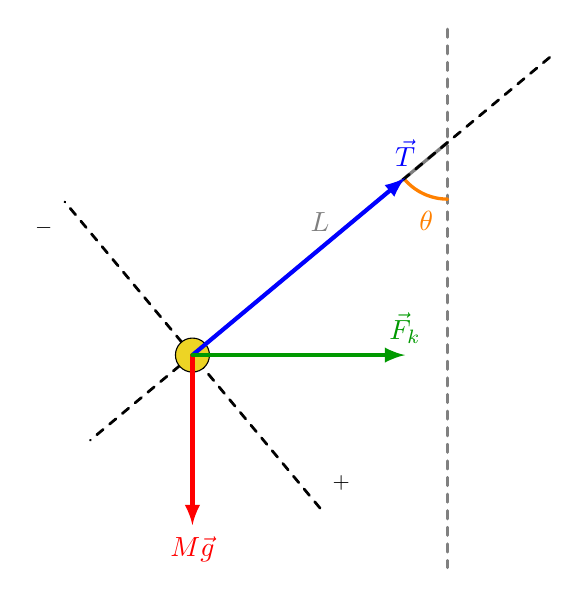
\begin{tikzpicture}[x=1.2cm,y=1.2cm,line cap=round,line join=round,>=latex,scale=1.5]
  % Coordenadas
  \coordinate (O) at (0,0);
  \coordinate (M) at (-1.8,-1.5);
  
  % Línea punteada vertical para referencia
  \draw[dashed,gray,line width=1pt] (0,0.8) -- (0,-3.0);
  
  % Ángulo theta
  \draw[thick,orange,line width=1.2pt] (0,-0.4) arc[start angle=-90, end angle=-140, radius=0.4];
  \node[orange] at (-0.15,-0.55) {$\theta$};
  
  % Línea desde origen a masa (cuerda)
  \draw[thick,gray,line width=1.2pt] (O) -- (M);
  \node[gray,above] at (-0.9,-0.7) {$L$};
  
  % Sistema de referencia inclinado con ángulo theta (líneas punteadas que se extienden en ambas direcciones)
  % Eje radial (perfectamente alineado con la cuerda O-M, extendido hacia el origen y más allá)
  \draw[dashed,black,line width=1pt] (0.72,0.60) -- (-2.52,-2.10);
  % Eje tangencial (perfectamente perpendicular al radial)  
  \draw[dashed,black,line width=1pt] (-0.9,-2.58) -- (-2.7,-0.42);
  
  % Convención de signos en el eje tangencial
  \node[black,scale=0.8] at (-0.75,-2.4) {$+$};
  \node[black,scale=0.8] at (-2.85,-0.6) {$-$};
  
  % Masa (redibujada para estar por encima de las líneas)
  \fill[yellow!70!brown, draw=black] (M) circle (0.12);
  
  % Fuerzas (dibujadas al final para que aparezcan por delante de todo)
  % Tensión T (por encima de la masa)
  \draw[->,thick,blue,line width=1.5pt] (M) -- ++(1.5,1.25) node[above] {$\vec{T}$};
  
  % Peso Mg
  \draw[->,thick,red,line width=1.5pt] (M) -- ++(0,-1.2) node[below] {$M\vec{g}$};
  
  % Fuerza del resorte
  \draw[->,thick,green!60!black,line width=1.5pt] (M) -- ++(1.5,0) node[above] {$\vec{F}_k$};
\end{tikzpicture}
\caption{Diagrama de fuerzas para el péndulo con resorte. La línea gris vertical punteada representa la posición de equilibrio. El ángulo $\theta$ (naranja) muestra el desplazamiento angular desde la vertical. Las líneas negras punteadas definen el sistema de coordenadas polares con eje radial alineado con la cuerda y eje tangencial perpendicular. Las fuerzas actuantes son: $\vec{T}$ (azul) tensión de la cuerda, $M\vec{g}$ (rojo) peso, y $\vec{F}_k$ (verde) fuerza del resorte, el sistema esta en la situacion en la que el sistema esta desacelerando y la fuerza elastica apunta a la derecha, por lo cual $a_{t} < 0 $}
\end{figure}
Por lo tanto  tenemos que en la direccion $\hat{x}$, recordemos que la aceleracion tangencial es $a_t = -L\ddot{\theta}$ (Dado la situacion de desaceleracion que estamos considerando) se debe cumplir que
\begin{align}
  a_{t} M &= P \cdot  \sin\theta + F_e \cdot L \cos\theta\\
  (-L\ddot{\theta})M &= P \cdot  \sin\theta + F_e \cdot L \cos\theta
\end{align}
Donde tenemos que:
\begin{align}
  F_{e} = kx(\cos(\theta)) = (k\sin\theta) \cos\theta
\end{align}
Donde el x es la elongacion del resorte en relacion al problema original, por lo que deberemos referenciarlo al nuevo sistema de coordenadas. De esta manera tenemos que:
\begin{align}
  -L\ddot{\theta}M = Mg\sin\theta - (kL \sin\theta) \cos\theta
\end{align}
Donde el signo negativo en la fuerza del resorte indica que se opone al desplazamiento. Dado que estamos en pequeñas oscilaciones, podemos hacer la aproximación $\sin\theta \approx \theta$ y $\cos\theta \approx 1$, con lo que el sistema resulta:
\begin{align}
  -L\ddot{\theta}M &= Mg\sin\theta - kL \sin\theta \cos\theta \\
  \Rightarrow -L\ddot{\theta}M &= Mg\,\overset{\theta}{\cancel{\sin\theta}} - kL\,\overset{\theta}{\cancel{\sin\theta}}\overset{1}{\cancel{\cos\theta}} \\
  -L\ddot{\theta}M &= Mg\theta - kL\theta \\
  -L\ddot{\theta}M - Mg\theta + kL\theta &= 0 \\
  ML\ddot{\theta} + Mg\theta - kL\theta &= 0 \\
  ML\ddot{\theta} + (Mg - kL)\theta &= 0 \\
  \Rightarrow \quad
  \ddot{\theta} + \frac{g}{L}\left(1 - \frac{kL}{Mg}\right)\theta = 0
\end{align}

Donde reconocemos corresponde a una ecuacion tipica de oscilador armonico simple, por lo que la frecuencia angular sera:
\begin{equation}
  \omega = \sqrt{\frac{g}{L}\left(1 + \frac{kL}{Mg}\right)}
\end{equation}
Por lo tanto el periodo de oscilacion sera:
\begin{equation}
  \boxed{T = 2\pi\sqrt{\frac{L}{g\left(1 + \frac{kL}{Mg}\right)}}}
\end{equation}

  \subsection*{Resolución 1.2}
  Dado los datos del problema los cuales son $M=1{,}00\,\mathrm{kg}$ y que el periodo del pendulo sin resorte es $T_0 = 2{,}00\,\mathrm{s}$ y el periodo con resorte es $T = 1{,}00\,\mathrm{s}$, debemos encontrar la constante elastica del resorte $k$. Para esto usaremos las expresiones del periodo obtenidas en la parte anterior y los datos entregados. Por lo que   el período del péndulo simple sin resorte:
  \begin{equation}
    T_0 = 2\pi\sqrt{\frac{L}{g}} = 2{,}00\
  \end{equation}
  De aquí podemos obtener el largo L dado por:
  \begin{align}
    L = g \left(\frac{T_0}{2\pi}\right)^2 = \left(\frac{2}{2\pi}\right)^2 = \frac{g}{\pi^2}\,
  \end{align}
  Con el resorte, tenemos que el período sera:
  \begin{equation}
    T = 2\pi\sqrt{\frac{L}{g\left(1 + \frac{kL}{Mg}\right)}} = 1{,}00\,\mathrm{s}
  \end{equation}
  
  Dividiendo las ecuaciones:
  \begin{equation}
    \frac{T}{T_0} = \frac{1}{\sqrt{1 + \frac{kL}{Mg}}} = \frac{1{,}00}{2{,}00} = \frac{1}{2}
  \end{equation}
  
  Elevando al cuadrado:
  \begin{equation}
    \frac{1}{4} = \frac{1}{1 + \frac{kL}{Mg}}
  \end{equation}
  
  Despejando:
  \begin{equation}
    1 + \frac{kL}{Mg} = 4 \quad \Rightarrow \quad \frac{kL}{Mg} = 3
  \end{equation}
  
  Por tanto:
  \begin{equation}
    k = \frac{3Mg}{L}
  \end{equation}
  
  Necesitamos encontrar $L$, tenemos que $L = \frac{g}{\pi^2}$:
  \begin{equation}
    L = \frac{g}{\pi^2} = \frac{9{,}81}{\pi^2} \approx 0{,}994\,\mathrm{m}
  \end{equation}
  
  Finalmente:
  \begin{equation}
    k = \frac{3 \times 1{,}00 \times 9{,}81}{0{,}994} \approx 29{,}6\,\mathrm{N/m}
  \end{equation}
  
  \begin{equation}
    \boxed{k \approx 29{,}6\,\mathrm{N/m}}
  \end{equation}
\end{solution}
%--------------------------
\question 
\begin{parts}
  \part Bosquee la función
  \begin{equation}
    f(x) = \frac{1\,\mathrm{cm}}{1 + \left(x/1\,\mathrm{cm}\right)^2}.
  \end{equation}
  Escriba $f(\bar{x})$ para $\bar{x} = x - ct$, donde $c$ es la velocidad de propagación de la onda y $t$ el tiempo. Si $c = 1\,\mathrm{cm/s}$, bosquee la función $u(x,t) = f(x-ct)$ para $t = 0, 1, 2\,\mathrm{s}$, donde $u(x,t)$ representa la amplitud de la onda en la posición $x$ y tiempo $t$.

  \part Calcule la velocidad vertical $v(x,t)$ de la cuerda en el instante $t = 0$. Para esto, derive la función $u(x,t)$ con respecto al tiempo considerando $x$ constante.

  \part Grafique $v(x,0)$ en función de $x$. Note que esta es positiva y negativa en ciertas partes. Interprete el resultado.
\end{parts}
%--------------------------
\begin{solution}
  \subsection*{Resolución 2.1}
  
Lo primero sera escribir la función $f(\bar{x})$ donde tenemos que c es la velocidad de propagacion de la onda. Tenemos que la funcion $f(x)$ original viene dada por:
  \begin{equation}
    f(x) = \frac{1\,\mathrm{cm}}{1 + \left(x/1\,\mathrm{cm}\right)^2}
  \end{equation}

  Para $\bar{x} = x - ct$, se tendra que la función se convierte en:
  \begin{equation}
    f(\bar{x}) = f(x-ct) = u(x,t) = \frac{1\,\mathrm{cm}}{1 + \left((x-ct)/1\,\mathrm{cm}\right)^2}
  \end{equation}
  
  Con $c = 1\,\mathrm{cm/s}$:
  \begin{align}
    u(x,t) &= \frac{1\,\mathrm{cm}}{1 + (x-t)^2/\mathrm{cm}^2} \\
    &= \frac{1\,\mathrm{cm}}{1 + (x-t)^2\,\mathrm{cm}^{-2}}
  \end{align}
  
  Para los tiempos específicos:
  \begin{align}
    t = 0\,\mathrm{s}: \quad u(x,0) &= \frac{1\,\mathrm{cm}}{1 + x^2\,\mathrm{cm}^{-2}} \\
    t = 1\,\mathrm{s}: \quad u(x,1) &= \frac{1\,\mathrm{cm}}{1 + (x-1\,\mathrm{cm})^2\,\mathrm{cm}^{-2}} \\
    t = 2\,\mathrm{s}: \quad u(x,2) &= \frac{1\,\mathrm{cm}}{1 + (x-2\,\mathrm{cm})^2\,\mathrm{cm}^{-2}}
  \end{align}
  
  El pulso se propaga hacia la derecha con velocidad $c = 1\,\mathrm{cm/s}$, manteniendo su forma. Esto se puede visualizar en lo siguiente:
  \begin{figure}[H]
    \centering
    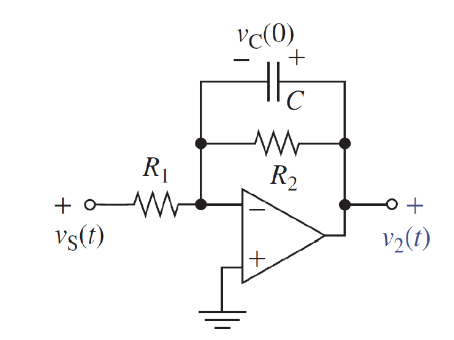
\includegraphics[width=0.6\textwidth]{Auxiliar_5_1}
    \caption{Gráfica de la función $u(x,t)$ en los tiempos $t = 0, 1, 2\,\mathrm{s}$. Se observa el pulso moviéndose hacia la derecha con velocidad constante.}
  \end{figure}
  
  \subsection*{Resolución 2.2}

Fijamos $x$ como constante y derivamos $u(x,t)$ respecto de $t$:
\begin{equation}
u(x,t) = \frac{1}{1+(x-ct)^2} = [1+(x-ct)^2]^{-1}
\end{equation}

Aplicamos la regla de la cadena, la cual se define como:
\begin{align}
\frac{d}{dt} f(g(t)) &= f'(g(t)) \cdot g'(t)
\end{align}
Para nuestro caso particular tenemos que:
\begin{align}
  f'(g(t)) &= -[1+(x-ct)^2]^{-2} \\
  g'(t) &= \frac{d}{dt}[1+(x-ct)^2]
\end{align}
Con lo que la derivada queda:
\begin{equation}
\frac{d}{dt} [1+(x-ct)^2]^{-1} = -[1+(x-ct)^2]^{-2} \cdot \frac{d}{dt}[1+(x-ct)^2]
\end{equation}

La derivada del corchete interior es:
\begin{align}
\frac{d}{dt}[1+(x-ct)^2] &= 2(x-ct) \cdot \frac{d}{dt}(x-ct) \\
&= 2(x-ct)(-c) \\
&= -2c(x-ct)
\end{align}

Por tanto, la velocidad vertical $v(x,t) = \frac{d}{dt}u(x,t)$ queda:
\begin{equation}
v(x,t) = -[1+(x-ct)^2]^{-2} \cdot [-2c(x-ct)] = \frac{2c(x-ct)}{[1+(x-ct)^2]^2}
\end{equation}

\begin{equation}
\boxed{v(x,t) = \frac{2c(x-ct)}{[1+(x-ct)^2]^2}}
\end{equation}

En $t=0$ y con $c=1\,\mathrm{cm/s}$:
\begin{equation}
\boxed{v(x,0) = \frac{2x}{(1+x^2)^2}}
\end{equation}




  \subsection*{Resolución 2.3}
  
  La función $v(x,0)$ tiene las siguientes características:
  
  \begin{itemize}
    \item Para $x > 0$: $v(x,0) > 0$ (velocidad hacia arriba)
    \item Para $x < 0$: $v(x,0) < 0$ (velocidad hacia abajo)  
    \item Para $x = 0$: $v(0,0) = 0$ (velocidad nula)
  \end{itemize}
  
  La velocidad máxima positiva ocurre en:
  \begin{equation}
    \frac{dv}{dx}\bigg|_{x=x_{\max}} = 0
  \end{equation}
  
  Resolviendo se obtiene $x_{\max} = 1/\sqrt{3}\,\mathrm{cm} \approx 0{,}577\,\mathrm{cm}$ con velocidad máxima:
  \begin{equation}
    v_{\max} = v\left(\frac{1}{\sqrt{3}}\,\mathrm{cm}, 0\right) = \frac{\sqrt{3}}{4}\,\mathrm{s}^{-1} \approx 0{,}433\,\mathrm{s}^{-1}
  \end{equation}
  
  Luego tenemos que la velocidad vertical describe cómo se mueve cada punto de la cuerda en el instante $t = 0$. El patrón antisimétrico ($v(-x,0) = -v(x,0)$) indica que el pulso se está propagando hacia la derecha. Los puntos a la derecha del centro se mueven hacia arriba (preparando el terreno para el pulso que llega), mientras que los puntos a la izquierda se mueven hacia abajo (regresando a la posición de equilibrio después de que el pulso ha pasado). Esto se visualiza en la siguiente gráfica:
  
  \begin{figure}[H]
    \centering
    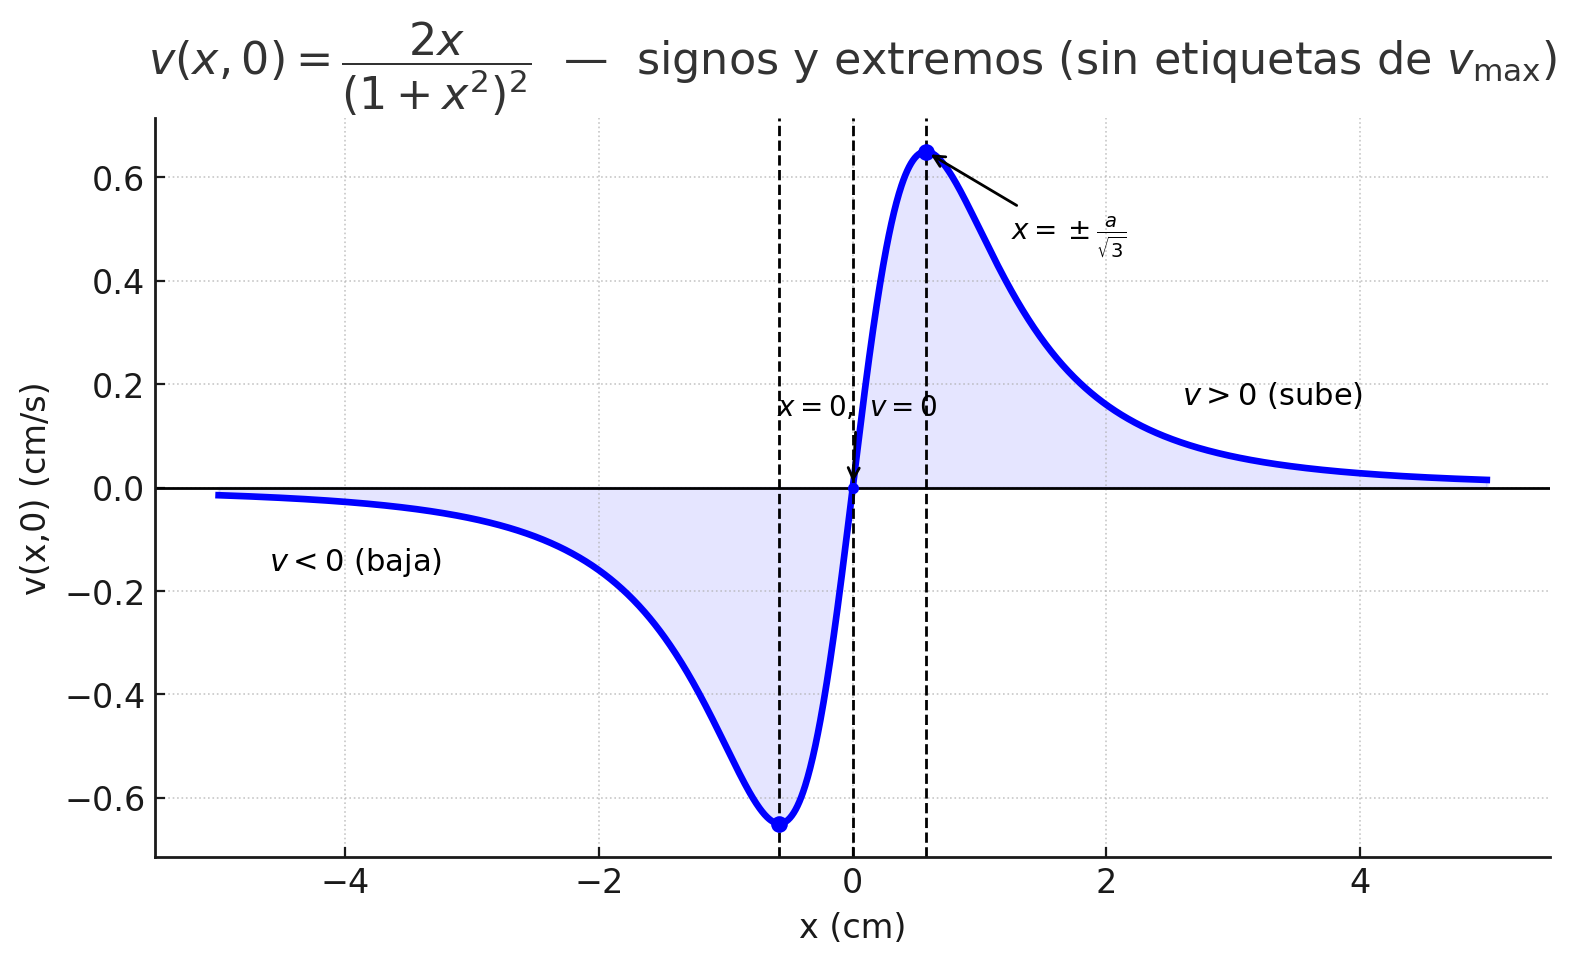
\includegraphics[width=0.8\textwidth]{Auxiliar_5_2}
    \caption{Gráfica de la velocidad vertical $v(x,0) = \frac{2x}{(1+x^2)^2}$ en función de la posición $x$. La función presenta características importantes: (1) \textbf{Antisimetría}: $v(-x,0) = -v(x,0)$, lo que indica propagación hacia la derecha. (2) \textbf{Punto de velocidad nula}: en $x = 0$, donde $v(0,0) = 0$. (3) \textbf{Velocidades extremas}: máxima positiva en $x = +a/\sqrt{3}$ y mínima negativa en $x = -a/\sqrt{3}$ (donde $a = 1\,\mathrm{cm}$). (4) \textbf{Interpretación física}: Los puntos con $x > 0$ se mueven hacia arriba ($v > 0$) preparando la llegada del pulso, mientras que los puntos con $x < 0$ se mueven hacia abajo ($v < 0$) regresando al equilibrio tras el paso del pulso. Esta distribución de velocidades es característica de ondas viajeras propagándose en la dirección positiva.}
  \end{figure}
\end{solution}

%--------------------------
\question Se tiene una masa $m$ sostenida de dos cuerdas de largos $L_1$ y $L_2$, con tensiones $T_1$ y $T_2$ respectivamente en presencia de gravedad, como se observa en la figura. Considere que $T_2$ es conocido y $T_1$ es tal que el sistema no se mueve verticalmente.

Si inicialmente la masa se suelta desde el reposo a una distancia $x$,
\begin{parts}
  \part Calcule el valor de $T_1$ para que el sistema no se mueva verticalmente.
  \part Encuentre la frecuencia angular de oscilación.
  \part Calcule el período de oscilación.
  \part Calcule la amplitud de oscilación de la masa.
\end{parts}
Considere para sus cálculos y aproximaciones $x \ll L_1, L_2$, y que las tensiones se mantienen al deformarse la cuerda.
\begin{figure}[H]
\centering
\begin{tikzpicture}[%
    >=Latex,
    board/.style={line width=2.6pt, draw=brown!70!black, line cap=round},
    stringV/.style={line width=1.4pt, draw=blue!70!black},
    string/.style={line width=1.4pt, draw=gray!70!black},
    mass/.style={draw=red!70!black, fill=red!70, line width=0.5pt},
    note/.style={scale=0.9}
]

% ------------------- Panel izquierdo: cuerda vertical -------------------
\def\H{3}    % altura entre barras
\def\W{3}    % ancho de barras
\def\xs{1}   % x de la cuerda
\def\ym{1.5} % y de la masa
\def\r{0.14} % radio de la masa

% Barras
\draw[board] (0,\H) -- (\W,\H);
\draw[board] (0,0)  -- (\W,0);

% Cuerda vertical
\draw[stringV] (\xs,0) -- (\xs,\H);

% Masa (por encima de la cuerda)
\fill[mass] (\xs,\ym) circle (\r);
\node[anchor=west] at (\xs+\r+0.08,\ym) {$m$};

% Tensiones T1 y T2
\node[note,blue!70!black,anchor=west] at (\xs+0.18, {(\H+\ym)/2}) {T1};
\node[note,blue!70!black,anchor=west] at (\xs+0.18, {\ym/2})      {T2};

% Brazos L1 y L2 con llaves
\draw[decorate,decoration={brace,mirror,amplitude=4pt}]
  ([xshift=-0.32cm]\xs,\ym) -- ([xshift=-0.32cm]\xs,\H)
  node[midway,left=6pt,note] {L1};
\draw[decorate,decoration={brace,mirror,amplitude=4pt}]
  ([xshift=-0.32cm]\xs,0) -- ([xshift=-0.32cm]\xs,\ym)
  node[midway,left=6pt,note] {L2};

% ------------------- Panel derecho: masa desplazada -------------------
\begin{scope}[xshift=6.2cm]
  % Barras
  \draw[board] (0,\H) -- (\W,\H);
  \draw[board] (0,0)  -- (\W,0);

  % Línea de referencia vertical
  \draw[stringV,dashed] (\xs,0) -- (\xs,\H);

  % Coordenadas clave
  \coordinate (Top) at (\xs,\H);
  \coordinate (Bot) at (\xs,0);
  \coordinate (M)   at (\xs+0.70,\ym); % masa desplazada

  % Cuerdas inclinadas (detrás de la masa)
  \draw[string] (Top) -- (M);
  \draw[string] (Bot) -- (M);

  % Etiquetas T1 y T2
  \node[note,anchor=west] at ($(Top)!0.58!(M)+(0.10,0.00)$) {T1};
  \node[note,anchor=west] at ($(Bot)!0.58!(M)+(0.10,0.00)$) {T2};

  % Flecha x (debajo de la masa y acortada al borde)
  \draw[->,thick,green!60!black,shorten >=\r+0.02]
    (\xs,\ym) -- (M) node[midway,above,note] {$x$};

  % Doble referencia L1/L2 (solo texto)
  \node[note] at (-0.35, {(\H+\ym)/2}) {L1};
  \node[note] at (-0.35, {\ym/2})      {L2};

  % Masa dibujada al final (encima de cuerdas y flecha)
  \fill[mass] (M) circle (\r);
  \node[anchor=west] at ($(M)+(\r+0.08,0)$) {$m$};
\end{scope}

% ------------------- Flecha de gravedad -------------------
\draw[->,line width=1.1pt] (11.0,2.6) -- (11.0,0.6) node[anchor=west] {$\vec g$};

\end{tikzpicture}
\caption{Masa sostenida por dos cuerdas con tensiones $T_1$ y $T_2$.}
\end{figure}
%--------------------------
\begin{solution}

\subsection*{Resolución 3.1}

Para que el sistema no se mueva verticalmente, debemos analizar el equilibrio de fuerzas en la dirección vertical.

Cuando la masa está desplazada horizontalmente una distancia $x$, las cuerdas forman ángulos $\theta_1$ y $\theta_2$ con la vertical, donde:
\begin{equation}
\sin\theta_1 = \frac{x}{\sqrt{x^2 + L_1^2}}, \qquad \cos\theta_1 = \frac{L_1}{\sqrt{x^2 + L_1^2}}
\end{equation}
\begin{equation}
\sin\theta_2 = \frac{x}{\sqrt{x^2 + L_2^2}}, \qquad \cos\theta_2 = \frac{L_2}{\sqrt{x^2 + L_2^2}}
\end{equation}

Para el equilibrio vertical (tomando positivo hacia arriba):
\begin{equation}
\sum F_y = T_1\cos\theta_1 - T_2\cos\theta_2 - mg = 0
\end{equation}

Sustituyendo las expresiones exactas:
\begin{equation}
T_1 \frac{L_1}{\sqrt{x^2 + L_1^2}} - T_2 \frac{L_2}{\sqrt{x^2 + L_2^2}} - mg = 0
\end{equation}

Esta ecuación relaciona las tensiones para cualquier posición $x$. En la posición de equilibrio ($x = 0$):
\begin{equation}
\boxed{T_1 = T_2 + mg}
\end{equation}

\subsection*{Resolución 3.2}

Para encontrar la frecuencia angular, analizamos las fuerzas horizontales restauradoras de manera general. Las componentes horizontales de las tensiones son:
\begin{align}
F_{1x} &= -T_1\sin\theta_1 = -T_1 \frac{x}{\sqrt{x^2 + L_1^2}} \\
F_{2x} &= -T_2\sin\theta_2 = -T_2 \frac{x}{\sqrt{x^2 + L_2^2}}
\end{align}

Para oscilaciones pequeñas alrededor del equilibrio, podemos expandir estas expresiones para $x \ll L_1, L_2$ usando la expansión de Taylor:
\begin{align}
\frac{x}{\sqrt{x^2 + L_i^2}} &= \frac{x}{L_i\sqrt{1 + (x/L_i)^2}} \\
&\approx \frac{x}{L_i} - \frac{x^3}{2L_i^3}
\end{align}

\textbf{Nota sobre aproximaciones paraxiales:} Si usáramos la aproximación paraxial ($\sin\theta \approx \theta$ y $\theta \approx \tan\theta = \frac{x}{L}$), obtendríamos directamente $\sin\theta \approx \frac{x}{L}$, lo que daría solo el término lineal. Esta aproximación es menos precisa que la expansión de Taylor, ya que omite los términos de orden superior que pueden ser importantes para analizar efectos no lineales, pero que para nuestro es suficiente. Por lo tanto, las fuerzas horizontales se aproximan como:
\begin{align}
F_{1x} &\approx -T_1 \left(\frac{x}{L_1} - \frac{x^3}{2L_1^3}\right) \\
F_{2x} &\approx -T_2 \left(\frac{x}{L_2} - \frac{x^3}{2L_2^3}\right)
\end{align}

Como se menciona anteriormente nos interesa solo las pequeñas oscilaciones, manteniendo solo el término lineal:
\begin{align}
F_{1x} &\approx -T_1 \frac{x}{L_1} \\
F_{2x} &\approx -T_2 \frac{x}{L_2}
\end{align}


Aplicando la segunda ley de Newton en la dirección horizontal (considerando solo términos lineales para MAS):
\begin{equation}
m\ddot{x} = F_{1x} + F_{2x} \approx -\left(\frac{T_1}{L_1} + \frac{T_2}{L_2}\right)x
\end{equation}


Para pequeñas oscilaciones, el término no lineal es despreciable ($x^3 \ll x$), por lo que obtenemos la ecuación del oscilador armónico simple:
\begin{equation}
m\ddot{x} = F_{1x} + F_{2x} = -\left(\frac{T_1}{L_1} + \frac{T_2}{L_2}\right)x
\end{equation}

Esta es la ecuación de un oscilador armónico simple:
\begin{equation}
\ddot{x} + \omega^2 x = 0
\end{equation}

donde:
\begin{equation}
\omega^2 = \frac{1}{m}\left(\frac{T_1}{L_1} + \frac{T_2}{L_2}\right)
\end{equation}

Sustituyendo $T_1 = T_2 + mg$:
\begin{equation}
\omega^2 = \frac{1}{m}\left(\frac{T_2 + mg}{L_1} + \frac{T_2}{L_2}\right) = \frac{T_2}{m}\left(\frac{1}{L_1} + \frac{1}{L_2}\right) + \frac{g}{L_1}
\end{equation}

\begin{equation}
\boxed{\omega = \sqrt{\frac{T_2}{m}\left(\frac{1}{L_1} + \frac{1}{L_2}\right) + \frac{g}{L_1}}}
\end{equation}

\subsection*{Resolución 3.3}

El período de oscilación es:
\begin{equation}
\boxed{T = \frac{2\pi}{\omega} = \frac{2\pi}{\sqrt{\frac{T_2}{m}\left(\frac{1}{L_1} + \frac{1}{L_2}\right) + \frac{g}{L_1}}}}
\end{equation}


\subsection*{Resolución 3.4}

Para un movimiento armónico simple, si la masa se suelta desde el reposo en la posición $x_0$, entonces:
- Posición inicial: $x(0) = x_0$
- Velocidad inicial: $\dot{x}(0) = 0$

La solución general del MAS es:
\begin{equation}
x(t) = A\cos(\omega t + \phi)
\end{equation}

Aplicando las condiciones iniciales:
\begin{align}
x(0) &= A\cos(\phi) = x_0 \\
\dot{x}(0) &= -A\omega\sin(\phi) = 0
\end{align}

De la segunda condición: $\sin(\phi) = 0$, por lo que $\phi = 0$ o $\phi = \pi$.

Si $\phi = 0$: $A = x_0$
Si $\phi = \pi$: $A = -x_0$

Como la amplitud es positiva por definición, tomamos $A = |x_0|$.

\begin{equation}
\boxed{A = |x_0| = |x|}
\end{equation}

donde $x$ es la distancia inicial desde la posición de equilibrio.
\end{solution}

\question En la siguiente figura se muestran dos pulsos, el pulso triangular se mueve hacia la derecha con una rapidez de $1~\mathrm{m/s}$ y el pulso rectangular se mueve hacia la izquierda también con una rapidez de $1~\mathrm{m/s}$. En el tiempo $t=0$, ambos pulsos están separados una distancia de $2~\mathrm{m}$.

\begin{enumerate}
  \item Considerando el sistema de referencia mostrado en la figura, escriba las funciones
  que representan al pulso triangular y al pulso rectangular por separado, para todo instante de tiempo.
  \item Dibuje el pulso resultante en los instantes $t=1,2,3,4~\mathrm{s}$. Considere que cuando
  dos ondas se encuentran, ambas ondas se suman.
\end{enumerate}

\begin{figure}[h!]
\centering
\begin{tikzpicture}[>=Stealth, scale=0.95]
  %----- Ejes
  \draw[->] (-0.4,0) -- (7.6,0) node[below] {$x$ (m)};
  \draw[->] (0,-0.25) -- (0,1.6) node[left] {$y$ (m)};

  %----- Marcas y valores en x
  \foreach \x in {0,1,2,3,4,5,6,7}{
    \draw (\x,0) -- (\x,-0.07) node[below] {\small \x};
  }
  % Marca en y=1 (y línea de referencia punteada)
  \draw (0,1) -- (-0.07,1) node[left] {\small 1};
  \draw[densely dotted] (0,1) -- (7,1);

  %----- Pulsos en t=0
  % Triangular (base 0..2, altura 1)
  \draw[line width=1.2pt] (0,0) -- (1,1) -- (2,0);
  % Rectangular (de 4 a 7, altura 1)
  \draw[line width=1.2pt] (4,0) -- (4,1) -- (7,1) -- (7,0);

  %----- Flechas de velocidad (1 m/s)
  \draw[->] (0.3,1.25) -- (1.8,1.25) node[midway, above] {\small $1~\mathrm{m/s}$};
  \draw[<-] (4.2,1.25) -- (6.8,1.25) node[midway, above] {\small $1~\mathrm{m/s}$};

  %----- Etiqueta t=0
  \node[right] at (7.1,1.02) {\small $t=0$};
\end{tikzpicture}
\caption{Condición inicial con marcas y valores en el eje $x$.}
\end{figure}
\begin{solution}

\subsection*{Resolucion 4.1 }

Denotemos por $f(x,t)$ el pulso triangular que viaja a la \emph{derecha} con rapidez $v$ y por $g(x,t)$ el pulso rectangular que viaja a la \emph{izquierda} con la misma rapidez $v$. A $t=0$: triángulo de altura $1$ sobre $[0,2]$ (vértice en $x=1$); rectángulo de altura $1$ sobre $[4,7]$.

Para un pulso que viaja sin deformarse:
\[
\text{derecha: } h(x,t)=h_0(x-vt),\qquad
\text{izquierda: } h(x,t)=h_0(x+vt).
\]

\textbf{Pulso triangular (derecha):}
\begin{equation}
f(x,t)=
\begin{cases}
0, & x<vt,\\[2pt]
x-vt, & vt\le x < 1+vt,\\[2pt]
2-(x-vt), & 1+vt\le x < 2+vt,\\[2pt]
0, & x\ge 2+vt.
\end{cases}
\end{equation}

\textbf{Pulso rectangular (izquierda):}
\begin{equation}
g(x,t)=
\begin{cases}
1, & 4-vt \le x \le 7-vt,\\[2pt]
0, & \text{en otro caso}.
\end{cases}
\end{equation}

En el problema $v=1~\mathrm{m/s}$. La superposición lineal es
\begin{equation}
y(x,t)=f(x,t)+g(x,t).
\end{equation}

\subsection*{Resolución 4.2}

Luego tenemos que de manera gráfica viene dada por:

\begin{figure}[H]
\centering
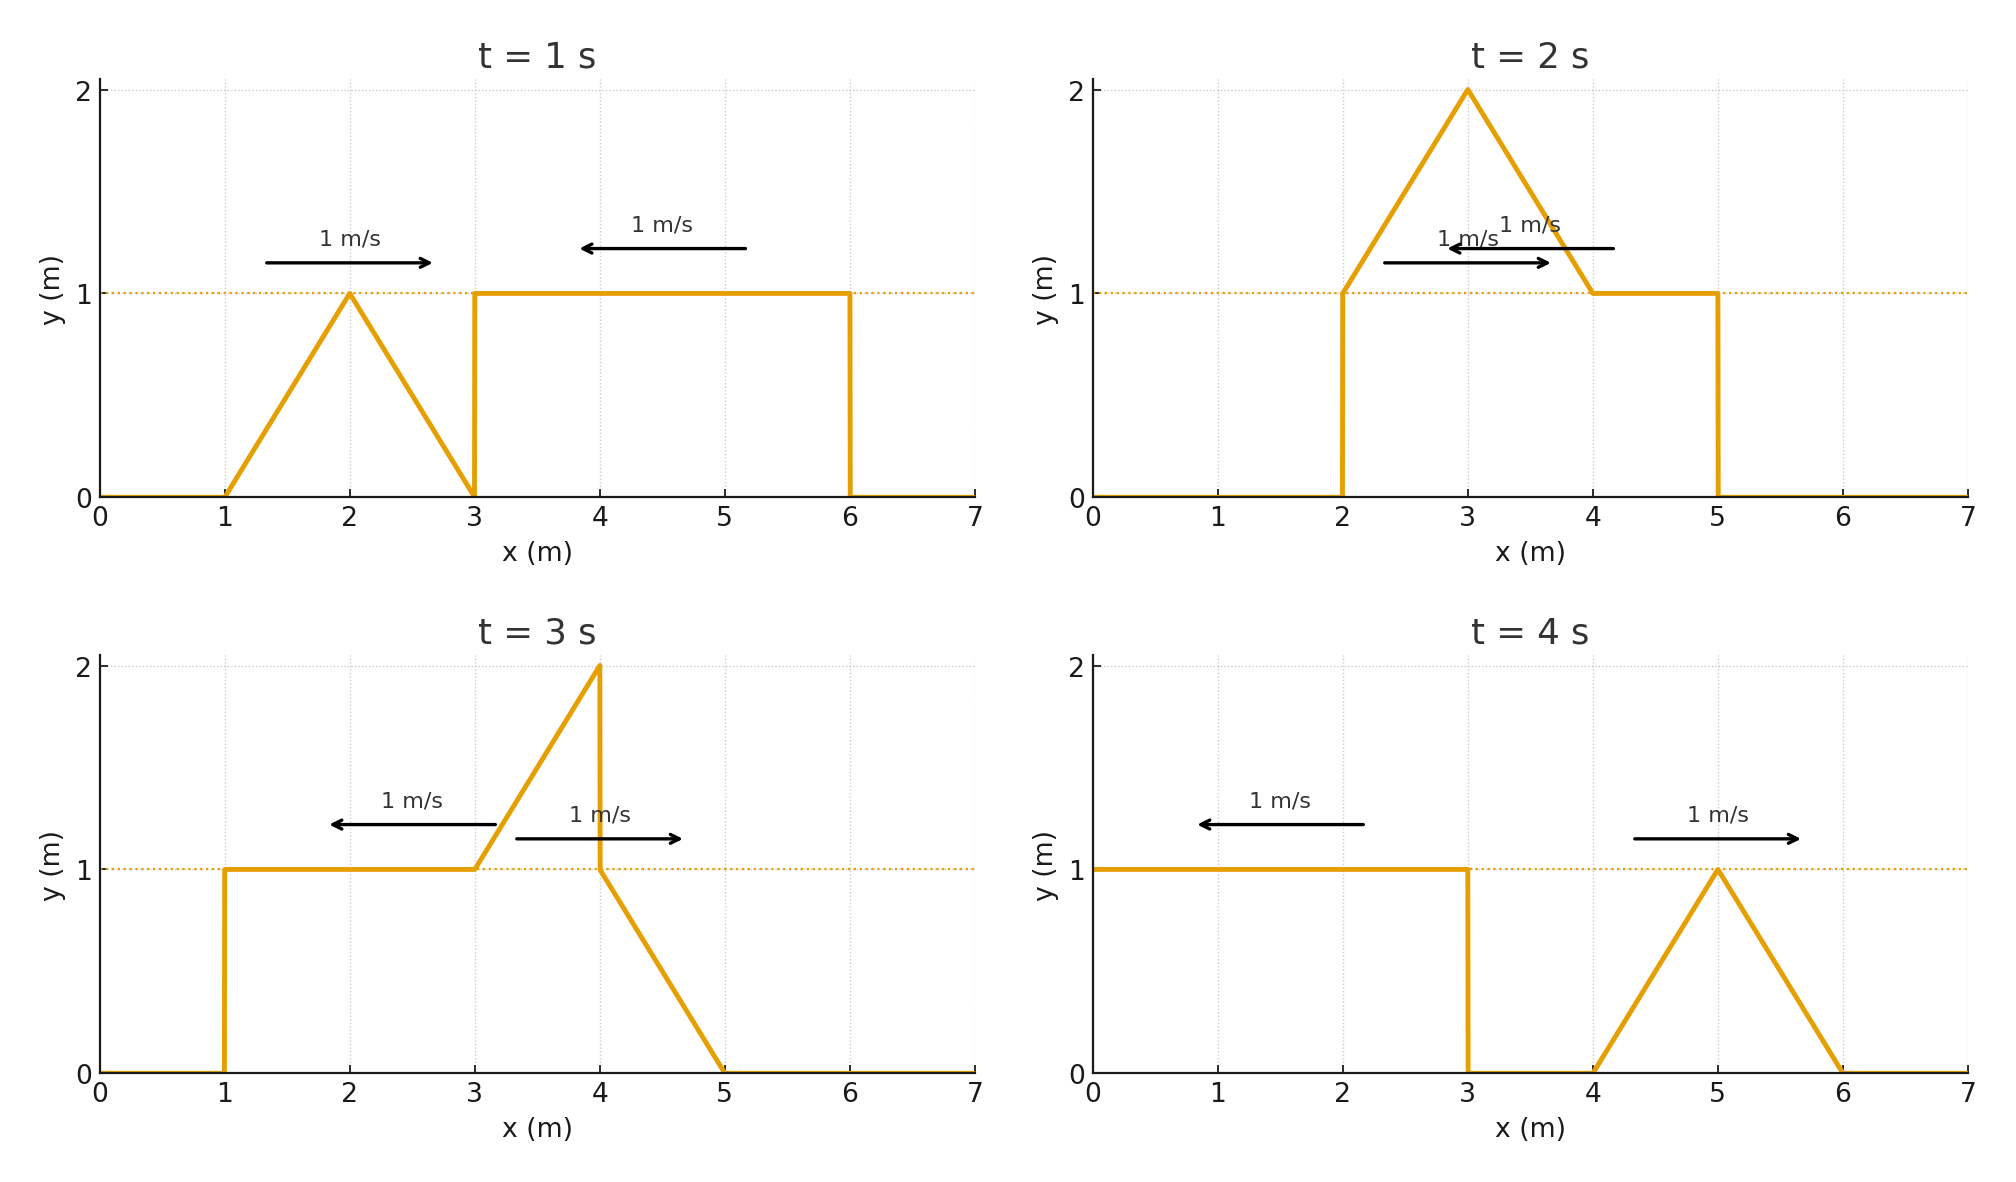
\includegraphics[width=\textwidth]{Auxiliar_5_3}
\caption{Superposición de los pulsos triangular y rectangular en diferentes instantes de tiempo. Se observa la propagación de ambos pulsos con velocidades opuestas de 1 m/s cada uno, y la interferencia constructiva cuando se superponen.}
\end{figure}

Luego podemos analizar cada instante de tiempo:
\begin{itemize}
\item \textbf{t = 1 s:} Los pulsos se han acercado. El pulso triangular se encuentra en el intervalo [1, 3] m con vértice en x = 2 m, mientras que el pulso rectangular ocupa [3, 6] m. Los pulsos están a punto de encontrarse en x = 3 m.

\item \textbf{t = 2 s:} Los pulsos se superponen parcialmente. El triángulo está en [2, 4] m y el rectángulo en [2, 5] m. En la región de superposición [2, 4] m, las amplitudes se suman constructivamente, resultando en valores mayores a 1 m en algunas regiones.

\item \textbf{t = 3 s:} Máxima superposición. El triángulo se encuentra en [3, 5] m y el rectángulo en [1, 4] m. La región de superposición [3, 4] m muestra la suma completa de ambas ondas, creando un patrón de interferencia complejo.

\item \textbf{t = 4 s:} Los pulsos se separan. El triángulo está en [4, 6] m y el rectángulo en [0, 3] m. Solo hay superposición mínima, y cada pulso continúa su propagación independiente manteniendo su forma original.
\end{itemize}

Este ejemplo ilustra perfectamente el principio de superposición lineal de ondas, donde la amplitud resultante en cualquier punto es la suma algebraica de las amplitudes individuales de cada onda. Después de la interacción, ambos pulsos emergen sin cambios en su forma original, demostrando que las ondas son fenómenos lineales que no se afectan permanentemente entre sí.
\end{solution}
%--------------------------
\question  Tres segmentos de cuerda de densidad $\mu$ están atados como muestra la figura. 
Suponga que se conocen las distancias $L_1$ y $L_2$, y el ángulo $\alpha$. 
Un pulso que parte en $A$ tarda un tiempo $T_B$ en llegar a $B$, y un tiempo $T_C$ en llegar a $C$. Encuentre la longitud de la cuerda $L_3$, y la tensión de la cuerda $L_1$.

\begin{figure}[h]
    \centering
    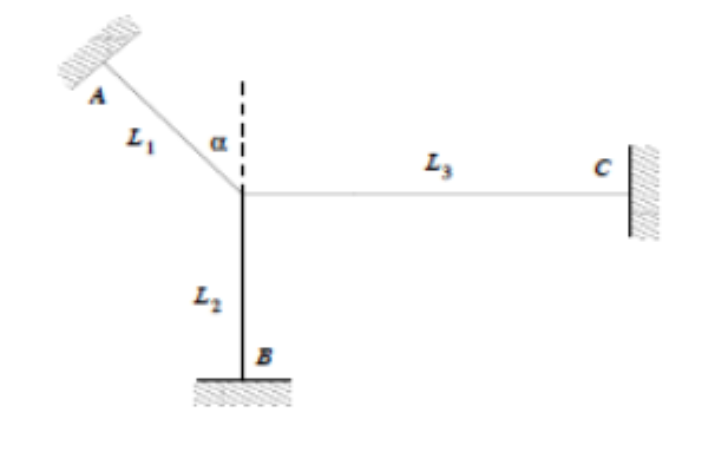
\includegraphics[width=0.5\textwidth]{Auxiliar_5_4}
    \caption{Esquema del sistema de cuerdas con segmentos $L_1$, $L_2$ y $L_3$ y ángulo $\alpha$.}
    \label{fig:cuerdas}
\end{figure}

\begin{solution}

\subsection*{Resolución 5.1}

Para resolver este problema, necesitamos analizar el equilibrio del nudo donde se unen las tres cuerdas y las condiciones de propagación del pulso, por lo que en el punto donde se unen las tres cuerdas, las fuerzas de tensión deben estar en equilibrio:
\begin{equation}
\vec{T}_1 + \vec{T}_2 + \vec{T}_3 = \vec{0}
\end{equation}

Considerando el sistema de coordenadas con $L_2$ vertical hacia abajo, $L_3$ horizontal hacia la derecha, y $\alpha$ el ángulo entre $L_1$ y la vertical, las componentes de equilibrio son:

\textbf{Equilibrio horizontal:}
\begin{equation}
T_1 \sin\alpha = T_3
\end{equation}

\textbf{Equilibrio vertical:}
\begin{equation}
T_1 \cos\alpha = T_2
\end{equation}

La velocidad de propagación en una cuerda está dada por $v = \sqrt{T/\mu}$, donde $T$ es la tensión y $\mu$ la densidad lineal. Por tanto:

\begin{align}
v_1 &= \sqrt{\frac{T_1}{\mu}} \\
v_2 &= \sqrt{\frac{T_2}{\mu}} = \sqrt{\frac{T_1 \cos\alpha}{\mu}} = v_1\sqrt{\cos\alpha} \\
v_3 &= \sqrt{\frac{T_3}{\mu}} = \sqrt{\frac{T_1 \sin\alpha}{\mu}} = v_1\sqrt{\sin\alpha}
\end{align}

El pulso que parte desde $A$ debe recorrer primero el segmento $L_1$ hasta el nudo, y luego continuar por el segmento correspondiente:

Para llegar a $B$:
\begin{equation}
T_B = \frac{L_1}{v_1} + \frac{L_2}{v_2} = \frac{L_1}{v_1} + \frac{L_2}{v_1\sqrt{\cos\alpha}} = \frac{1}{v_1}\left(L_1 + \frac{L_2}{\sqrt{\cos\alpha}}\right)
\end{equation}

Para llegar a $C$:
\begin{equation}
T_C = \frac{L_1}{v_1} + \frac{L_3}{v_3} = \frac{L_1}{v_1} + \frac{L_3}{v_1\sqrt{\sin\alpha}} = \frac{1}{v_1}\left(L_1 + \frac{L_3}{\sqrt{\sin\alpha}}\right)
\end{equation}

De la ecuación para $T_B$:
\begin{equation}
v_1 = \frac{L_1 + \frac{L_2}{\sqrt{\cos\alpha}}}{T_B}
\end{equation}

Sustituyendo en la ecuación para $T_C$:
\begin{equation}
T_C = \frac{L_1 + \frac{L_3}{\sqrt{\sin\alpha}}}{\frac{L_1 + \frac{L_2}{\sqrt{\cos\alpha}}}{T_B}}
\end{equation}

Despejando $L_3$:
\begin{equation}
\boxed{L_3 = \sqrt{\sin\alpha}\left[\frac{T_C}{T_B}\left(L_1 + \frac{L_2}{\sqrt{\cos\alpha}}\right) - L_1\right]}
\end{equation}


Usando $v_1 = \sqrt{T_1/\mu}$:
\begin{equation}
T_1 = \mu v_1^2 = \mu \left(\frac{L_1 + \frac{L_2}{\sqrt{\cos\alpha}}}{T_B}\right)^2
\end{equation}

\begin{equation}
\boxed{T_1 = \frac{\mu}{T_B^2}\left(L_1 + \frac{L_2}{\sqrt{\cos\alpha}}\right)^2}
\end{equation}
Las tensiones en los otros segmentos son:
- $T_2 = T_1 \cos\alpha$
- $T_3 = T_1 \sin\alpha$

Estas relaciones confirman que el equilibrio del nudo se mantiene con las tensiones calculadas.
\end{solution}
%--------------------------
\end{questions}
\end{document}